\chapter{EDA Lab IV: Titanic (Interactions and Text Features) and Pima Diabetes (Disguised Missing Values)}
\companion{Kaggle: Titanic, Machine Learning from Disaster (search)}{\yts{titanic+dataset+EDA+pandas+seaborn+tutorial}}

Two more \textbf{real} datasets from your repository, each chosen for one lesson interviewers love: Titanic for interactions, feature extraction from text
and group-wise imputation; Pima diabetes for missing values that \code{isna()} cannot see. Notebook sections: \emph{Case 3} and \emph{Case 4}.

\section{Titanic: who survived?}
\subsection{Overview}
\begin{lstlisting}
ti = load_csv("understanding_your_data_eda/train.csv"); overview(ti)
\end{lstlisting}
\outlabel
\begin{lstlisting}[style=out]
(891, 12)
               dtype  missing  missing_%  n_unique                  example
PassengerId    int64        0        0.0       891                        1
Survived       int64        0        0.0         2                        0
Pclass         int64        0        0.0         3                        3
Name             str        0        0.0       891  Braund, Mr. Owen Harris
Sex              str        0        0.0         2                     male
Age          float64      177       19.9        88                     22.0
SibSp            int64        0        0.0         7                        1
Parch            int64        0        0.0         7                        0
Ticket           str        0        0.0       681                A/5 21171
Fare         float64        0        0.0       248                     7.25
Cabin            str      687       77.1       147                      C85
Embarked         str        2        0.2         3                        S
\end{lstlisting}
Note that \code{Pclass} is stored as an integer but is an \emph{ordinal category}; \code{Name} and \code{Ticket} are text that may hide features; \code{Cabin} is 77\% missing.

\subsection{Sex and class, and their interaction}
\begin{lstlisting}
print("survival rate:", ti["Survived"].mean().round(3))
rate_by(ti, "Sex", "Survived"); rate_by(ti, "Pclass", "Survived")
pd.crosstab(ti["Pclass"], ti["Sex"], values=ti["Survived"], aggfunc="mean").round(3)
\end{lstlisting}
\outlabel
\begin{lstlisting}[style=out]
survival rate: 0.384
Sex: female 0.742 (314) | male 0.189 (577)          Pclass: 1 0.630 (216) | 2 0.473 (184) | 3 0.242 (491)
Sex     female   male
Pclass
1        0.968  0.369
2        0.921  0.157
3        0.500  0.135
\end{lstlisting}
\begin{center}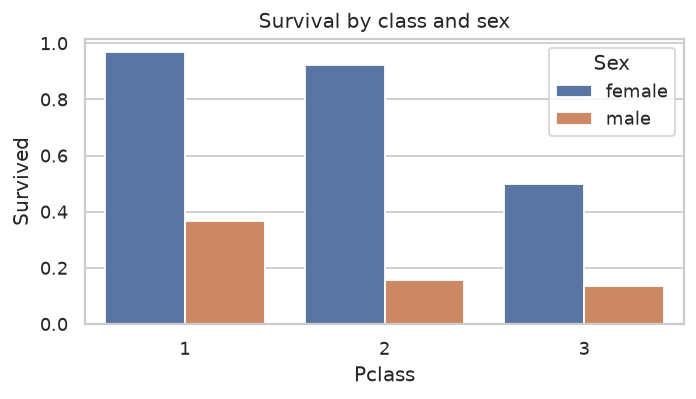
\includegraphics[width=0.55\linewidth]{eda_lab/figs/ti_class_sex.png}\end{center}
\textbf{Reading}: sex is the dominant factor (74\% vs 19\%), class the second. But the effect of class \textbf{depends on} sex: for women, moving from 2nd to 3rd class halves survival
(92\% to 50\%); for men the big drop is from 1st to 2nd (37\% to 16\%). That is an \textbf{interaction}. A decision tree finds it automatically; a logistic regression needs an
explicit \code{Sex}$\times$\code{Pclass} feature.

\subsection{Extracting a feature from text: the title}
\begin{lstlisting}
ti["Title"] = ti["Name"].str.extract(r",\s*([^\.]+)\.")[0]          # "Braund, Mr. Owen" -> "Mr"
ti["Title"] = ti["Title"].replace({"Mlle": "Miss", "Ms": "Miss", "Mme": "Mrs"})
ti.loc[~ti["Title"].isin(["Mr", "Mrs", "Miss", "Master"]), "Title"] = "Rare"
ti.groupby("Title").agg(n=("Survived", "size"), survival=("Survived", "mean"), median_age=("Age", "median"))
\end{lstlisting}
\outlabel
\begin{lstlisting}[style=out]
          n  survival  median_age
Master   40      0.57         3.5
Miss    185      0.70        21.0
Mr      517      0.16        30.0
Mrs     126      0.79        35.0
Rare     23      0.35        48.5
\end{lstlisting}
\textbf{Reading}: the title combines sex, age and status in one feature: ``Master'' means a boy (median age 3.5), and boys survived at 57\% while men (``Mr'') survived at 16\%.
The regular expression reads ``after a comma and spaces, capture everything up to the first full stop''.

\subsection{Group-wise imputation of Age}
\begin{lstlisting}
ti["Age_filled"] = ti["Age"].fillna(ti.groupby("Title")["Age"].transform("median"))
print("global median age:", ti["Age"].median(), "| ages imputed:", ti["Age"].isna().sum())   # 28.0, 177
\end{lstlisting}
Filling all 177 missing ages with the global median 28 would turn missing boys into adults and erase the ``children first'' pattern; filling by title gives boys 3.5 and married women
35. (In a modelling pipeline compute the medians on training folds only.)

\subsection{Fare, family size and cabin}
\begin{lstlisting}
print("Fare skew:", ti["Fare"].skew().round(2), "| log1p skew:", np.log1p(ti["Fare"]).skew().round(2),
      "| zero fares:", (ti["Fare"] == 0).sum())
ti["FamilySize"] = ti["SibSp"] + ti["Parch"] + 1
rate_by(ti, "FamilySize", "Survived", bins=[0, 1, 4, 11])
ti.groupby(ti["Cabin"].isna())["Survived"].mean()
\end{lstlisting}
\outlabel
\begin{lstlisting}[style=out]
Fare skew: 4.79 | log1p skew: 0.39 | zero fares: 15
(0, 1]    0.304  537        (1, 4]  0.579  292        (4, 11]  0.161   62
survival if Cabin missing vs present: {False: 0.667, True: 0.3}
\end{lstlisting}
\begin{center}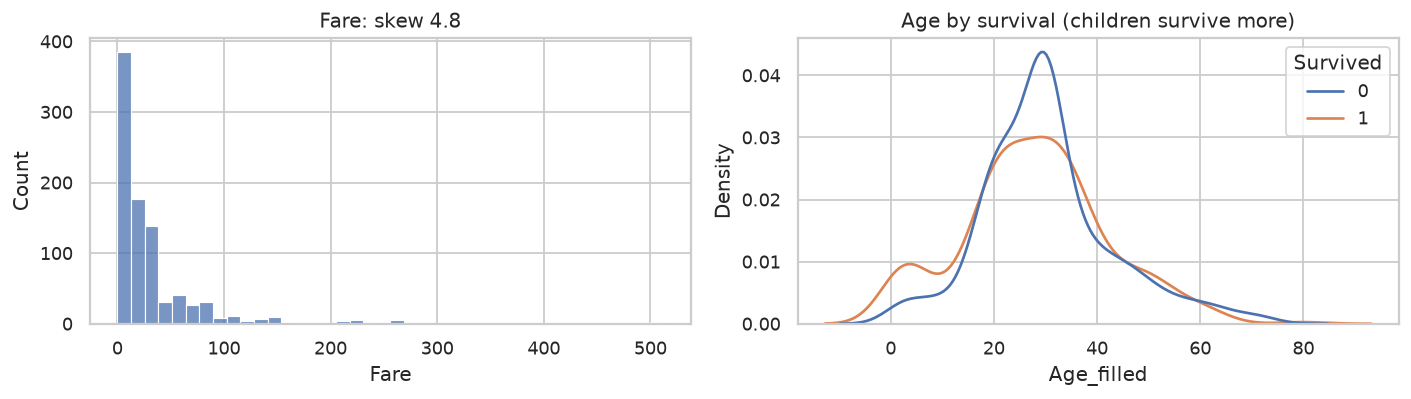
\includegraphics[width=\linewidth]{eda_lab/figs/ti_fare_age.png}\end{center}
\textbf{Reading}:
\begin{itemize}
\item \code{Fare} is extremely right-skewed (4.8; max 512): log it for linear models. Fifteen zero fares are suspicious (crew? complimentary tickets?): investigate, do not silently keep
  them as real prices.
\item \textbf{Family size is non-monotonic}: alone 30\%, 2--4 people 58\%, 5 or more 16\%. A linear term would miss it; bins or trees capture it. This is an engineered feature
  (\code{SibSp + Parch + 1}) that is more meaningful than its parts.
\item Missing \code{Cabin} goes with 30\% survival versus 67\% when present: cabin numbers were recorded mostly for first-class passengers, so missingness encodes class
  (informative, MNAR-like). Use ``has cabin'' as a feature rather than imputing cabins.
\item The age KDE shows the survival advantage concentrated among young children.
\end{itemize}

\subsection{Titanic findings}
Sex $\gg$ class with a strong interaction; title is a powerful compact feature; impute age by title; log fare and check zero fares; family size is non-monotonic; cabin missingness is
informative; \code{Embarked} has 2 missing values (fill with the mode, harmless). A depth-limited tree or gradient boosting will capture the interactions; logistic regression needs
engineered interaction terms.

\section{Pima Indians diabetes: missing values in disguise}
\subsection{The dataset says it has no missing values}
\begin{lstlisting}
pi = load_csv("Module_1_Foundation_of_ML_AI/dataset/diabetes.csv")
print(pi.shape, "| isna().sum() total:", pi.isna().sum().sum())
num_summary(pi)
\end{lstlisting}
\outlabel
\begin{lstlisting}[style=out]
(768, 9) | isna().sum() total: 0
                count    mean     std   min    25%    50%     75%    max  skew  kurt  n_iqr_outliers  n_zeros
Pregnancies     768.0    3.85    3.37  0.00   1.00   3.00    6.00   17.0  0.90  0.16               4      111
Glucose         768.0  120.89   31.97  0.00  99.00  117.00  140.25  199.0  0.17  0.64               5        5
BloodPressure   768.0   69.11   19.36  0.00  62.00   72.00   80.00  122.0 -1.84  5.18              45       35
SkinThickness   768.0   20.54   15.95  0.00   0.00   23.00   32.00   99.0  0.11 -0.52               1      227
Insulin         768.0   79.80  115.24  0.00   0.00   30.50  127.25  846.0  2.27  7.21              34      374
BMI             768.0   31.99    7.88  0.00  27.30   32.00   36.60   67.1 -0.43  3.29              19       11
DiabetesPedigreeFunction 768 0.47  0.33  0.08   0.24    0.37    0.63    2.42  1.92  5.59              29        0
Age             768.0   33.24   11.76 21.00  24.00   29.00   41.00   81.0  1.13  0.64               9        0
Outcome         768.0    0.35    0.48  0.00   0.00    0.00    1.00    1.0  0.64 -1.60               0      500
\end{lstlisting}
\textbf{Reading the clues}: \code{min = 0} for Glucose, BloodPressure, SkinThickness, Insulin and BMI. A living person cannot have a blood pressure, BMI or glucose of 0. The
\code{n\_zeros} column counts them: 374 Insulin, 227 skin thickness, 35 blood pressure, 11 BMI, 5 glucose. BloodPressure's skew of $-1.84$ and kurtosis 5.2 are artefacts of the
spike at 0. These are \textbf{missing values coded as 0}. (Zero pregnancies is valid.)

\subsection{Recode and re-examine}
\begin{lstlisting}
impossible_zero = ["Glucose", "BloodPressure", "SkinThickness", "Insulin", "BMI"]
pi2 = pi.copy(); pi2[impossible_zero] = pi2[impossible_zero].replace(0, np.nan)
(pi2.isna().mean() * 100).round(1)
pi2.groupby("Outcome").median().round(1).T
point_biserial(pi2, pi2.columns.drop("Outcome"), "Outcome")
\end{lstlisting}
\outlabel
\begin{lstlisting}[style=out]
missing %: Glucose 0.7 | BloodPressure 4.6 | SkinThickness 29.6 | Insulin 48.7 | BMI 1.4
medians by outcome after fixing:              point-biserial with Outcome:
Outcome                     0      1           Glucose 0.495 | BMI 0.314 | Insulin 0.303 | SkinThickness 0.260
Glucose                 107.0  140.0           Age 0.238 | Pregnancies 0.222 | Pedigree 0.174 | BloodPressure 0.171
BloodPressure            70.0   74.5
SkinThickness            27.0   32.0
Insulin                 102.5  169.5
BMI                      30.1   34.3
Age                      27.0   36.0
\end{lstlisting}
\begin{center}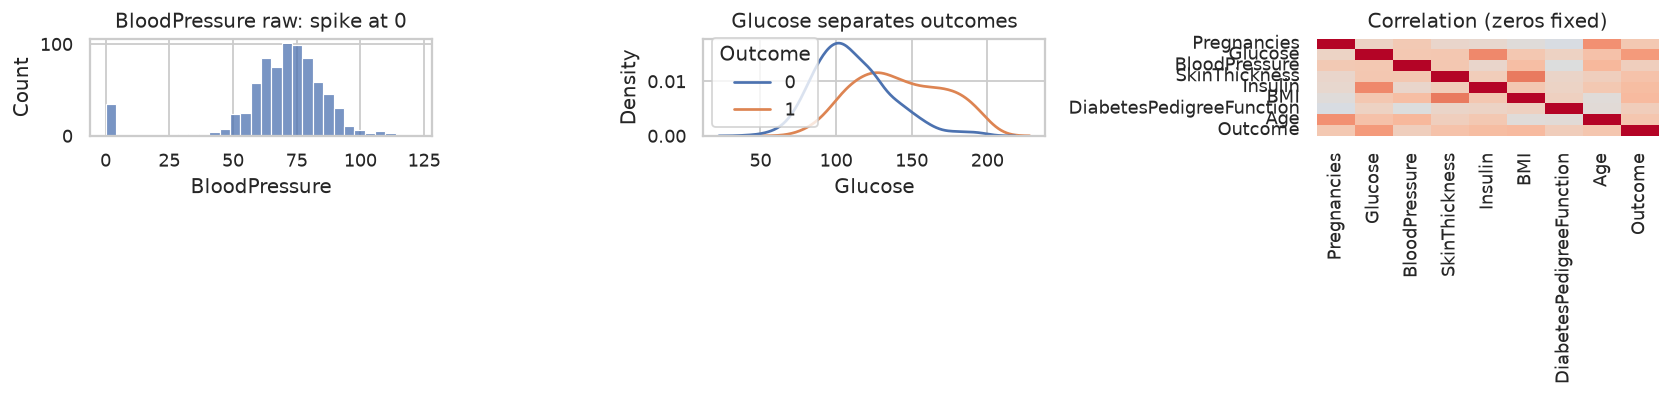
\includegraphics[width=\linewidth]{eda_lab/figs/pi_overview.png}\end{center}
\textbf{Reading}:
\begin{itemize}
\item Insulin is missing for almost half the patients (48.7\%) and skin thickness for 30\%: these columns need careful imputation or a missing indicator.
\item \textbf{The trap}: with the zeros left in, the median insulin of diabetic patients is \textbf{0} (more than half were simply not measured), suggesting the absurd conclusion that
  diabetics have no insulin. After recoding, diabetic patients have \emph{higher} median insulin (169.5 vs 102.5), as expected with insulin resistance.
\item Glucose is the dominant predictor ($r = 0.50$; medians 140 vs 107); then BMI and insulin ($\approx0.3$), age and pregnancies.
\item The blood-pressure histogram's spike at 0 is the visual signature of disguised missingness; always look at histograms, not just \code{isna()}.
\end{itemize}
\textbf{Imputation plan}: median or KNN/iterative imputation computed on training folds only, \emph{without} using the outcome; add missing indicators for Insulin and SkinThickness;
compare model performance with and without those two columns.

\stuck{Kaggle: Pima Indians Diabetes Database (search)}{\yts{pima+indians+diabetes+EDA+zero+values+missing}}
\section{Interview questions}

\begin{qa}{\deep The Pima dataset has no NaN values. Why is that misleading, and how did you detect the problem?}
\oneline{Missing measurements were stored as 0; I detected them because \code{describe()} shows minimum 0 for glucose, blood pressure, skin thickness, insulin and BMI (physically impossible), the zero
counts are large, and histograms show spikes at 0; recoding them as NaN reveals 48.7\% missing insulin.}
\why The consequence of ignoring it: means are biased downward, distributions distorted, and the diabetic patients' median insulin appears to be 0.
\end{qa}

\begin{qa}{Explain the sex--class interaction in Titanic and how different models handle it.}
\oneline{Class matters differently for each sex (women: 97\%, 92\%, 50\% across classes; men: 37\%, 16\%, 14\%); trees and boosting learn this through successive splits, while logistic
regression, being additive in log-odds, needs an explicit \code{Sex}$\times$\code{Pclass} interaction feature.}
\end{qa}

\begin{qa}{How would you impute Titanic's missing ages, and why not the global median?}
\oneline{By the median age of the passenger's title (Master 3.5, Miss 21, Mr 30, Mrs 35), computed on training data; the global median (28) would turn missing boys into adults and weaken the
strong child-survival pattern.}
\end{qa}

\begin{qa}{Cabin is 77\% missing. Drop it?}
\oneline{Drop the raw cabin string, but keep ``has cabin'' (survival 67\% vs 30\%), because missingness encodes passenger class and wealth; the deck letter can also be extracted where present.}
\end{qa}

\begin{qa}{What does a non-monotonic relationship like family size vs survival imply for modelling?}
\oneline{A single linear coefficient cannot represent a rise-then-fall pattern (alone 30\%, 2--4 58\%, 5+ 16\%); use bins, polynomial or spline terms, or tree-based models.}
\end{qa}

\begin{qa}{Write the pandas code to extract the title from a name like ``Braund, Mr. Owen Harris''.}
\oneline{\code{df["Name"].str.extract(r",\textbackslash s*([\textasciicircum\textbackslash .]+)\textbackslash .")[0]}: after the comma and optional spaces, capture characters that are not a full stop,
up to the first full stop.}
\end{qa}

\begin{qa}{\deep Across the four datasets, what are the recurring EDA lessons?}
\oneline{Check how a value was recorded before trusting it (salary after placement, cabins for first class, zeros for unmeasured insulin); relate missingness to the target; look for
non-linear and interaction effects with binned rates and pivots; extract features from text; and never call a value an outlier without a domain range.}
\end{qa}
